Notre base de données est constituée de 4 tables:
\vspace*{0.5cm}
\begin{itemize}
    \item Une table \texttt{Utilisateur} stockant les informations des joueurs. Ses colonnes sont : \texttt{idUser} qui est l’identifiant du joueur de type entier, son nom d'utilisateur \texttt{pseudo} de type str, un mot de passe \texttt{motDePasse} de type str et un sel  \texttt{salt} pour la sécurisation du compte utilisateur. La chaîne de caractères stockée dans la colonne \texttt{motDePasse} sera le haché de la concaténation du mot de passe et du salt.
     \vspace*{0.2cm}
    
    \item Une table \texttt{Partie} qui stocke les données des parties jouées de chaque joueur connecté. Ses colonnes sont : \texttt{idPartie} qui représente l’identifiant d’une partie de type int, \texttt{idUser} qui est une clé étrangère référençant l'identifiant de l'utilisateur, les points d'expérience \texttt{pts\_experience} de type int qui représentent les points gagnés lors d’une partie, le mot à deviner \texttt{motSecret} associé à la partie de type str, le nombre d'essais utilisés par le joueur pour trouver le mot secret \texttt{nb\_coups} de type int, le nombre d’essais maximum de la partie \texttt{nb\_essais\_maximum} de type int, la longueur des mots associée au mot de la partie \texttt{longueur\_mot} de type int et le mode de jeu défini par le joueur \texttt{modejeu} (mode sans fin ou mode classique).
     \vspace*{0.2cm}
    
    \item Une table \texttt{AchievementDesc} qui stocke les descriptions des achievements. Ses colonnes sont : \texttt{idSucces} qui est l’identifiant de l’achievement et \texttt{description} la description associée : gagner une partie en 3 coups ou moins, gagner 10 parties, etc\dots{}
     \vspace*{0.2cm}
    
    \item Une table \texttt{Achievements} qui relie les tables \texttt{AchievementDesc} et \texttt{Partie} dont les colonnes sont : \texttt{idPartie}, clé étrangère qui référence l'identifiant d'une partie et \texttt{idSucces}, clé étrangère référençant l'identifiant d'un achievement. Ces 2 clés forment la clé primaire de la table \texttt{Achievements}.
\end{itemize}

Notre base de données est en 3ème forme normale.

\begin{figure}[h!]
    \centering
    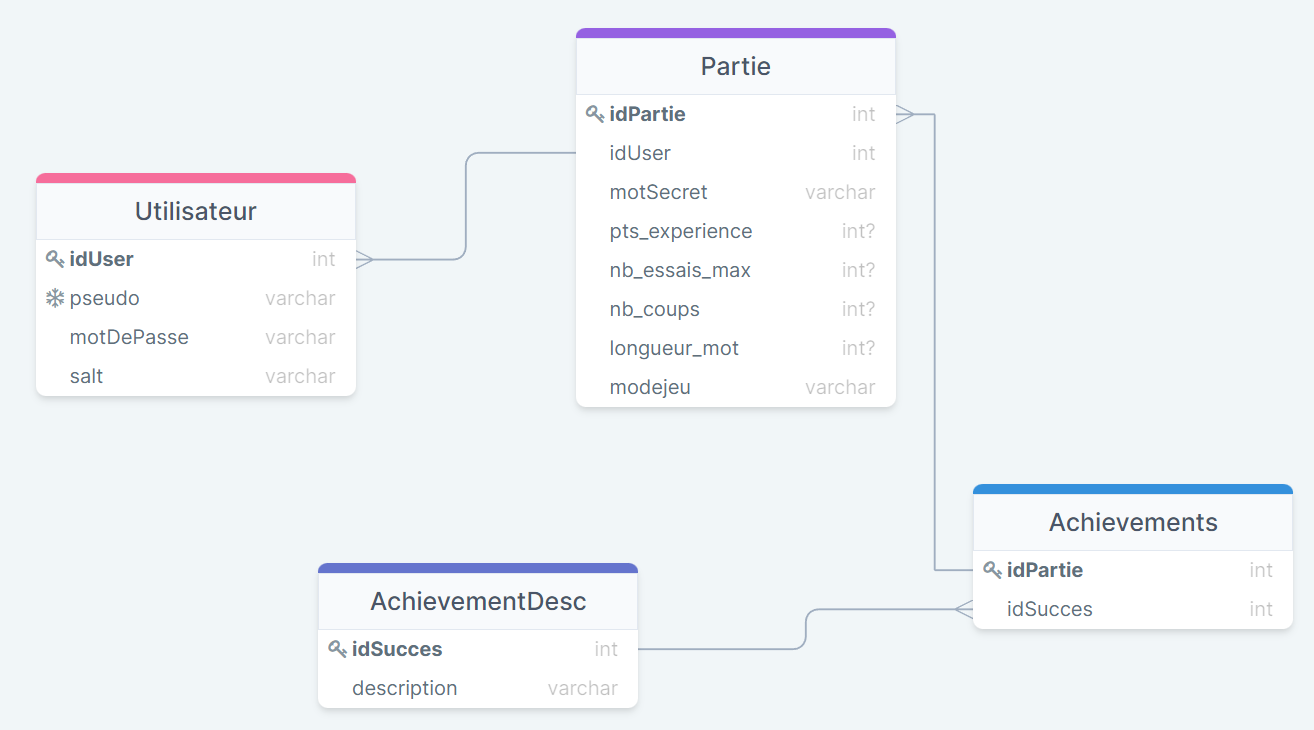
\includegraphics[width=16cm]{figures/bddfinale.PNG}
    \caption{Schéma de la base de données de WORDLE}
\end{figure}

\begin{figure}[h!]
    \centering
    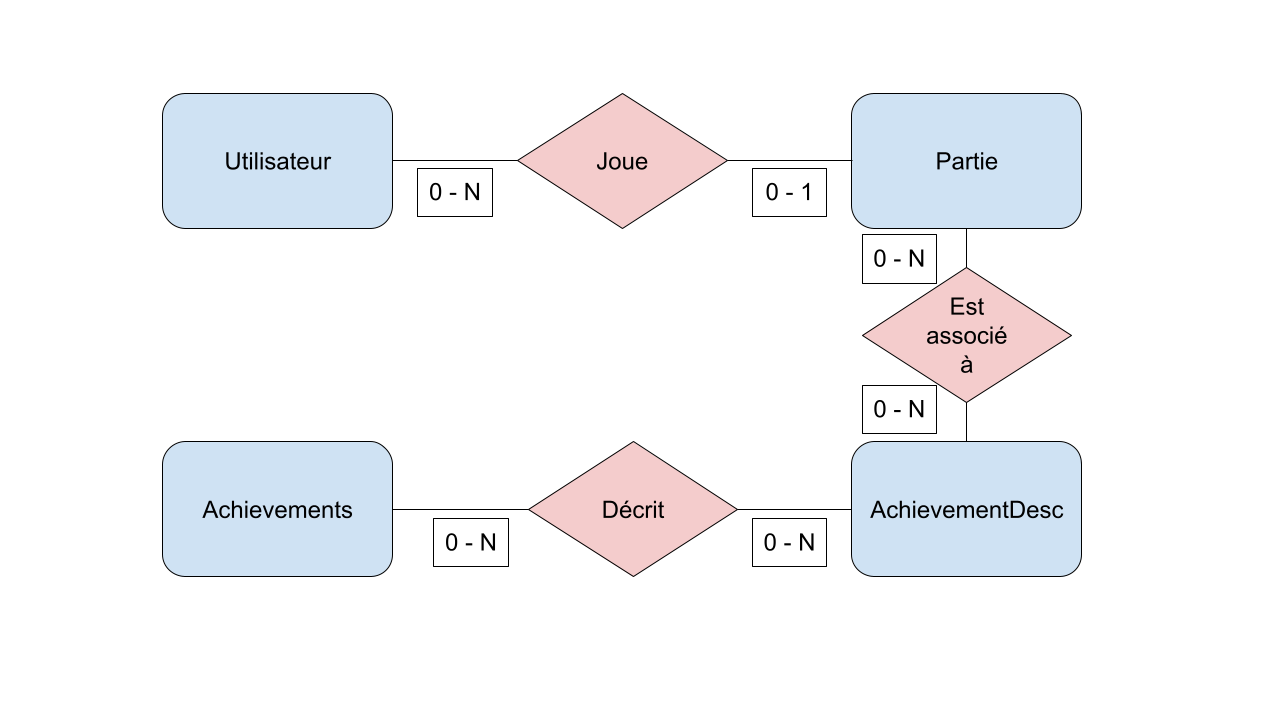
\includegraphics[width=16cm]{figures/modele_entite_association.png}
    \caption{Modèle entité-association de la base de données}
\end{figure}